\subsection{Page conditioning and line segmentation}
\label{sec:segmentation}

This block turns a photograph of a handwritten page into clean, deskewed, white-background line images for the text recogniser of Section~\ref{sec:textrec} and the writer classifier of Section~\ref{sec:writerid}. It covers functional units FU~2.1 and FU~2.2 and serves requirement R2.

The deployed implementation is \texttt{SegmentLean.py}, which is eleven functions in about 570 lines behind a single entry point, \texttt{SegmentLines(path)}. The web server, the style-profile builder and the writer-classifier trainer all call that same entry point, so training pages are cut by exactly the code that cuts a page during normal use. Published methods are cited where they are used, and the rules around them are plain array arithmetic written for this project.

No part of this block resamples through an imaging library. Every operation that changes a pixel value --- the $2{:}1$ page reduction, the deskew rotation, the background enlargement of Equation~\ref{eq:seg-flat} and the four mask enlargements of stage~6 --- is performed by the project's own module, which implements Equation~\ref{eq:seg-resize} directly. The library is used only to read the file from disk and to write the optional debug overlay. Each of those replacements was verified against the library call it replaced, and the results are in Section~\ref{sec:seg-test}.

\subsubsection{Design goals and the measured scale unit}

A flat-bed scan can be conditioned by grey conversion, binarisation and bounding-box line separation, which is what published pipelines do~\cite{hemanth2022,chen2023}. A photograph is harder. It adds uneven illumination, the surroundings of the sheet, skew, printed rules, edge slivers, creases, and lines that touch each other.

The block therefore has three design goals. It must work at any camera resolution and any handwriting size without manual tuning, it must never delete handwriting in order to remove a nuisance, and it must keep as few fixed constants as possible.

The way all three are met is to let the page set its own scale. The photograph is first reduced $2{:}1$ per axis by box averaging, which keeps thin pale strokes that point sampling would drop. The \emph{line pitch} $P$ is then measured on that working image in stage~5. Almost every later threshold is a multiple of $P$, so the same code works on a 2\,megapixel and an 8\,megapixel photograph without changing a number. Only four constants are absolute: the blur radius, the floor of 60 ink pixels per emitted line, the $64\times640$ canvas size and the dynamic-program weights. Table~\ref{tab:seg-const} in Appendix~\ref{sec:app-seg} lists every minor constant with the reason for its value.

\paragraph{The geometry of a line of handwriting.}
\label{sec:seg-geom}
Every subsystem from here onwards measures handwriting against the same five quantities, so they are defined once here and used unchanged for the rest of Section~\ref{sec:design}. They are the standard typographic reference lines of a line of writing, shown in Figure~\ref{fig:seg-geom}.

The \emph{baseline} is the line the body of the lower-case letters sits on. The \emph{x-height} $x_{\mathrm{h}}$ is the height of a lower-case letter that has neither a tall part nor a tail, such as x, o or e, measured up from the baseline. An \emph{ascender} is the part of a letter such as h, l or b that reaches above the x-height, and a \emph{descender} is the part of a letter such as p, g or y that falls below the baseline. The \emph{line pitch} $P$ is the distance from one baseline to the next.

Two of these five are used as units, and which one is used depends on what is being measured. The pitch $P$ is the unit of this block, because segmentation is about separating one line from the next and every threshold here is a fraction of a line spacing. The x-height $x_{\mathrm{h}}$ is the unit of everything downstream of this block: the writer classifier redraws ink at a pen width proportional to it (Section~\ref{sec:wid-strokenorm}), the style builder stores every glyph in a frame scaled by it (Section~\ref{sec:styleprofile}), and the synthesiser converts back to millimetres by one multiplication at the very end (Section~\ref{sec:synthesis}).

The reason for using the writing's own geometry as the unit, rather than pixels or millimetres, is that it removes two variables at once. A page photographed closer to the camera has more pixels per letter but the same number of x-heights per letter, and a writer with large handwriting has more millimetres per letter but, again, the same number of x-heights. Measuring in x-heights therefore makes every stored style parameter independent of both the camera and the size the writer happens to write at, which is what allows one style profile to be drawn at any pen size.

The ascender reach $A$ and descender reach $D$ are stored per writer as multiples of $x_{\mathrm{h}}$, with $A>1$ because an ascender reaches above the x-height line and $D<0$ because a descender falls below the baseline. A \emph{ligature} is the connecting stroke a writer draws between two joined letters, and it matters later because it is the only place in joined handwriting where one letter honestly ends and the next begins (Section~\ref{sec:styleprofile}).

\begin{figure}[h]
\centering
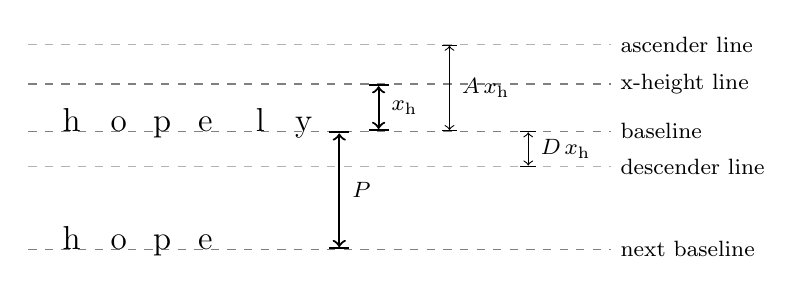
\begin{tikzpicture}[x=1cm,y=1cm,font=\footnotesize]
%% reference lines of the first text line
\draw[dashed,gray]      (0,0)    -- (7.4,0)    node[right,black]{baseline};
\draw[dashed,gray]      (0,0.6)  -- (7.4,0.6)  node[right,black]{x-height line};
\draw[dashed,gray!60]   (0,1.1)  -- (7.4,1.1)  node[right,black]{ascender line};
\draw[dashed,gray!60]   (0,-0.45)-- (7.4,-0.45)node[right,black]{descender line};
%% letters placed against those lines: h has an ascender, x and o do not, p descends
\node[anchor=base,font=\large] at (0.55,0) {h};
\node[anchor=base,font=\large] at (1.15,0) {o};
\node[anchor=base,font=\large] at (1.70,0) {p};
\node[anchor=base,font=\large] at (2.25,0) {e};
\node[anchor=base,font=\large] at (2.95,0) {l};
\node[anchor=base,font=\large] at (3.50,0) {y};
%% x-height dimension
\draw[|<->|,thick] (4.45,0) -- (4.45,0.6) node[midway,right=1pt]{$x_{\mathrm{h}}$};
%% ascender and descender reach, measured from the baseline in x-heights
\draw[|<->|] (5.35,0) -- (5.35,1.1)  node[midway,right=1pt]{$A\,x_{\mathrm{h}}$};
\draw[|<->|] (6.35,0) -- (6.35,-0.45)node[midway,right=1pt]{$D\,x_{\mathrm{h}}$};
%% second text line, to show the pitch
\draw[dashed,gray] (0,-1.5) -- (7.4,-1.5) node[right,black]{next baseline};
\node[anchor=base,font=\large] at (0.55,-1.5) {h};
\node[anchor=base,font=\large] at (1.15,-1.5) {o};
\node[anchor=base,font=\large] at (1.70,-1.5) {p};
\node[anchor=base,font=\large] at (2.25,-1.5) {e};
\draw[|<->|,thick] (3.95,0) -- (3.95,-1.5) node[midway,right=1pt]{$P$};
\end{tikzpicture}
\caption{The five quantities every subsystem measures handwriting against. The x-height $x_{\mathrm{h}}$ is the height of a lower-case letter with no tall part and no tail; an ascender reaches above it and a descender below the baseline. The ascender and descender reaches $A$ and $D$ are stored as multiples of $x_{\mathrm{h}}$, so $A>1$ and $D<0$. The line pitch $P$ is the baseline-to-baseline distance and is the unit used by this block; $x_{\mathrm{h}}$ is the unit used by every block after it.}
\label{fig:seg-geom}
\end{figure}

Ink is described in two tiers. A strict page-wide mask fixes the structure of the page, such as where the paper is and where the lines are. A second, more permissive threshold is then applied inside each individual crop, limited to a halo around that line's own strong ink, which recovers pale strokes that the strict mask missed. The reason for two tiers is that a threshold loose enough to catch a faint stroke is also loose enough to catch a shadow, so the loose threshold is only trusted next to ink that is already known to belong to that line.

The six stages are reduce, ink mask, deskew, clean-up, pitch and centres, and finally seams and crops. They are described in that order below, which is the order the data flows through them.

Three of the stages resample an image, and they do it by bilinear interpolation at the source position given by Equation~\ref{eq:seg-resize}. The exception is one ownership map, which uses nearest neighbour, because the values in that map are integer line indices and interpolating them would invent indices that do not exist. Equation~\ref{eq:seg-clf} is the scale used to paste a finished crop onto the white $640\times64$ canvas that both networks expect, flush left and vertically centred.
\begin{align}
y_s&=\frac{(i+0.5)\,h}{h'}-0.5,\quad x_s=\frac{(j+0.5)\,w}{w'}-0.5,\quad I'(i,j)=\sum_{a,b\in\{0,1\}}\omega_{ab}\,I(\lfloor y_s\rfloor+a,\lfloor x_s\rfloor+b),\label{eq:seg-resize}\\
s&=\min\!\Bigl(\frac{64}{h},\frac{640}{w}\Bigr),\qquad h'=\max(1,\mathrm{round}(hs)),\qquad w'=\max(1,\mathrm{round}(ws)).\label{eq:seg-clf}
\end{align}
The single scale factor $s$ in Equation~\ref{eq:seg-clf} is applied to both axes, so letter proportions are not distorted. Flushing the crop left has a second benefit that Section~\ref{sec:styleprofile} depends on: the map from a network time step back to a pixel column of the original crop is then the exact inverse $x_{\mathrm{orig}}=x_{\mathrm{canvas}}/s$, with no offset to track.

Each line record that the block returns holds the order index, the crop at native resolution, that canvas, and the bounding box in full-resolution coordinates. The block also returns page statistics: the chosen skew angle, the pitch, the paper coverage, the ink discarded off the paper, the straight pixels and artefact pieces removed, the line count and the wall-clock time. These allow a page to be checked after the fact without having to instrument the module.

\subsubsection{The three array primitives}

Almost every operation in this block is a sum, a maximum, or a test of whether anything is set, taken over a rectangular window. Computed directly, a window of radius $r$ costs $O(r)$ per pixel per axis. That is too slow here, because the illumination blur below uses a radius of up to 40 pixels.

The module therefore builds a summed-area table~\cite{crow1984}, also called an integral image, which is Equation~\ref{eq:seg-sat}. It is built in one $O(HW)$ pass of two cumulative sums, and after that the sum over a window of \emph{any} size costs four look-ups instead of $(2r+1)^2$ additions. The window corners are $y_2=y_1+2r+1$ and $x_2=x_1+2r+1$. The array is padded by $r$ using edge replication first, so that every window holds the same number of samples and a pixel near the border is not biased.
\begin{align}
S(y,x)&=\sum_{i<y}\sum_{j<x} I(i,j),\qquad
\mathrm{BoxSum}=S(y_2,x_2)-S(y_1,x_2)-S(y_2,x_1)+S(y_1,x_1),\label{eq:seg-sat}\\
\mathrm{AnyWithinRadius}&(m,r)[i]=\bigl[\,c[i+2r+1]-c[i]>0\,\bigr]=\Bigl[\textstyle\bigvee_{k=-r}^{r} m[i+k]\Bigr],\label{eq:seg-dilate}\\
\mathrm{LongRun}&(m,n)[j]=\bigl[\,\mathrm{ch}[h_j+1]-\mathrm{ch}[l_j]>0\,\bigr],\ l_j=\max(0,j-n+1),\ h_j=\min(j,L-n).\label{eq:seg-runmask}
\end{align}
The second primitive, Equation~\ref{eq:seg-dilate}, is a dilation. A square dilation separates into two one-axis dilations, and each of those is a cumulative sum of the mask followed by one subtraction, so it also costs the same at any radius. An erosion is then the complemented dilation of the complement, and a closing is a dilation followed by an erosion, which means no other structuring element has to be implemented.

The third primitive, Equation~\ref{eq:seg-runmask}, marks every pixel that lies on a run of at least $n$ consecutive set pixels. A run of length $n$ starts at position $i$ exactly when $c[i+n]-c[i]=n$, so the starts are found first and then a second cumulative sum marks every pixel covered by one. This is what stage~4 uses to find printed rules. Figure~\ref{fig:seg-primspseudo} gives all three primitives as pseudocode.

Only one true Gaussian filter is used in the whole block, and it smooths the row profile in stage~5. It is a 25-tap kernel $k[t]\propto\exp(-t^2/2\sigma^2)$ for $t=-12\ldots12$ with $\sigma=4$ rows, truncated at $3\sigma$ and normalised. Four rows is about a tenth of a typical pitch, so it smooths the ripple inside a line without blurring one line into the next.

\subsubsection{Stage 2: lighting normalisation and the ink mask}

The intensity measured by a camera is approximately the reflectance of the paper multiplied by the illumination falling on it. Because the unwanted term is a multiplication and not an addition, it is divided out rather than subtracted. The working grey image $G$ is divided by a single box mean of itself, which is Equation~\ref{eq:seg-flat}. The result is a ratio image $\rho$ which is close to 1 on paper whatever the lighting, and on ink is the ink-to-paper reflectance ratio of the pen itself.
\begin{align}
\rho(p)&=\frac{G(p)}{\max\bigl(\mathrm{BoxMean}_r(G)(p),\,1\bigr)},\qquad r=\max\bigl(8,\;\min(40,\;\mathrm{round}(H/41))\bigr),\label{eq:seg-flat}\\
t^*&=\arg\max_t\;\omega_B(t)\,\omega_F(t)\,\bigl[\mu_B(t)-\mu_F(t)\bigr]^2 .\label{eq:seg-otsu}
\end{align}
The radius $r$ in Equation~\ref{eq:seg-flat} scales with the image height, so the background estimate covers the same fraction of the page at any resolution. It must be much larger than a letter, otherwise the letters would darken their own background estimate and disappear.

Once the shading has been divided out, the ink decision is a single global threshold, and Otsu's method~\cite{otsu1979} is used to choose it. Otsu's threshold is the value that maximises the between-class variance of Equation~\ref{eq:seg-otsu}, where $\omega_B$ and $\omega_F$ are the fractions of samples below and above $t$ and $\mu_B$ and $\mu_F$ are their means. A pixel is marked as ink when $\rho<t^*$. The cumulative form of Equation~\ref{eq:seg-otsu} is evaluated for all 256 histogram bins at once rather than in a loop.

A single global threshold is only possible because of the division. This is the step that removed the long chain of clean-up filters that the project's first segmenter needed, and it is why this stage holds no tunable grey level at all. One extra test is still needed: a solid-area veto removes any window that is entirely ink, because no pen stroke fills a $9\times9$ window. That catches a binder shadow or the dark gutter of a bound book, which a global threshold would otherwise mark as ink. The whole stage is four array statements, given as pseudocode in Figure~\ref{fig:seg-inkpseudo}.

\subsubsection{Stage 3: deskew by searching rotations}

When the text lines are horizontal, the row-sum profile of the ink has sharp peaks at the line bodies and deep troughs between them. Any tilt smears those peaks, because a single row then cuts across several lines. The sharpness of the profile is therefore a measure of how level the page is, and it can be maximised directly.

A candidate angle is scored by the projection objective of Equation~\ref{eq:seg-skew}, in which $R_\theta$ is the ink mask rotated by $\theta$.
\begin{equation}
J(\theta)=\sum_y P_\theta(y)^2,\qquad P_\theta(y)=\sum_x R_\theta(y,x),\qquad \theta^*=\arg\max_\theta J(\theta).
\label{eq:seg-skew}
\end{equation}
Squaring the profile before summing is what makes Equation~\ref{eq:seg-skew} work. The total amount of ink does not change when the page is rotated, so $\sum_yP_\theta(y)$ is fixed and could not be used. The sum of squares is largest when the same ink is concentrated into the fewest rows, which happens when the lines are level.

The search is one sweep of 17 candidate angles from $-4^\circ$ to $+4^\circ$ in steps of $0.5^\circ$, scored on the stage-2 mask reduced by a further factor of two. There is no refinement pass, so the best accuracy the stage can reach is half a step, which is $0.25^\circ$.

The page is never actually rotated to score an angle, which is worth setting out because it is what makes the sweep affordable. Rotating a point by $\theta$ about the centre of the image puts it in row
\begin{equation}
k=(y-c_y)\cos\theta-(x-c_x)\sin\theta+c_y,
\label{eq:seg-skewrow}
\end{equation}
so the coordinates of the ink pixels can be mapped straight into row numbers by Equation~\ref{eq:seg-skewrow} and counted, which gives the profile $P_\theta$ of Equation~\ref{eq:seg-skew} without producing a rotated image at all. That is one pass over the ink pixels per angle instead of seventeen image rotations, measured at 31 times faster, and it avoids resampling the mask seventeen times, each of which would blur it slightly further and bias the comparison towards the angles evaluated last.

One detail of that counting is not optional. Ink that would fall outside the row range at a trial angle must be allowed to extend the profile rather than being clipped into the first or last row. Clipping piles every out-of-range pixel into a single row, and because the objective squares each row, that artificial spike scores higher than any real text line; it made the search choose an angle four degrees wrong on a tilted page before it was corrected.

Only once an angle is chosen is the page itself rotated, bilinearly, and the ink mask and ratio image are then recomputed, because Equation~\ref{eq:seg-flat} is not rotation-equivariant: rotating the page and then dividing does not give the same result as dividing and then rotating.

The first segmenter had a fault here that is worth recording, because the structure of the deployed stage prevents it. A sign mismatch between the rotation routine and the angle scorer meant the page was rotated the wrong way, which doubled the skew of every tilted page instead of removing it. The deployed module cannot have that fault, because the candidate masks are rotated by the very same call that is later applied to the page, so the two cannot disagree about the sign. Section~\ref{sec:seg-test} measures what the stage actually achieves.

\subsubsection{Stage 4: removing what is not handwriting}

A first pitch $P$ is computed by the procedure of stage~5, and every threshold in this stage is a multiple of it. Three kinds of nuisance are then removed in turn.

The first is the area outside the sheet. Handwriting disappears under a coarse enough average while the sheet itself does not, and that is what separates them. The working image is block-averaged down, blurred, and thresholded against its own median, after which the largest bright connected component is taken to be the sheet and is eroded slightly to keep its darkened rim out of the ink mask. The result is reported as \texttt{paperCoverage} and \texttt{inkOutsidePaper}.

The second is printed structure. Ruled paper, underlines and the spine shadow of a bound book weld separate text lines into one piece of ink, which would defeat the line separation entirely. What distinguishes them from handwriting is that they run straight for longer than a line spacing, and handwriting does not. The long-run primitive is therefore applied per axis, bracketed by a dilation and a re-intersection as in Equation~\ref{eq:seg-cand}, where $\mathcal D_r^{y}$ and $\mathcal D_r^{x}$ are one-axis dilations.
\begin{equation}
\begin{aligned}
\mathrm{flat}&=\mathcal D_{1}^{y}\Bigl(\mathrm{LongRun}^{x}\bigl(\mathcal D_{1}^{y}(\mathrm{ink}),\;\lfloor1.25P\rfloor\bigr)\Bigr)\wedge\mathrm{ink},\\
\mathrm{upright}&=\mathcal D_{3}^{x}\Bigl(\mathrm{LongRun}^{y}\bigl(\mathcal D_{3}^{x}(\mathrm{ink}),\;\lfloor1.4P\rfloor\bigr)\Bigr)\wedge\mathrm{ink}.
\end{aligned}
\label{eq:seg-cand}
\end{equation}
The dilation before the run test is what makes Equation~\ref{eq:seg-cand} tolerant of a slight tilt, because a rule that drifts by one row would otherwise break into runs too short to detect. The re-intersection with the ink mask afterwards means only real ink is ever removed, never the pixels the dilation added. The two run lengths, $1.25P$ horizontally and $1.4P$ vertically, are the essential point: both are longer than any single letter can be, so no letter can be mistaken for a rule.

The third kind of nuisance is edge slivers, corner shadows and fold creases, which survive the run test because they are not straight. These are judged as whole pieces instead of pixel by pixel, because what identifies them is a property of the whole shape, such as being long and thin or being sparse inside its own bounding box.

Doing that requires the ink to be grouped into pieces first, which is \emph{connected-component labelling}: every set pixel is given an integer label, and two pixels get the same label when a path of set pixels joins them. The mask is closed before labelling so that the pen lifts inside a word are bridged and a whole word becomes one piece rather than several. The labelling itself is done by a run-length union-find pass. Each row is first reduced to its horizontal runs of set pixels, which is far fewer objects than pixels, and a \emph{union-find} structure then records which runs have been found to belong together: it holds one representative per group and merges two groups in near-constant time when a run in one row is found to touch a run in the next. One pass over the rows therefore labels the whole page.

Every statistic used by the discard tests is then accumulated over the \emph{original} ink pixels rather than the closed mask, so the closing can join pieces but can never add area to a decision. Eight discard predicates are applied to each piece, combining its size, its aspect ratio, its faintness relative to the page's own threshold, and its distance from the frame. Table~\ref{tab:seg-artifact} in Appendix~\ref{sec:app-seg} states all eight with the nuisance each is meant to catch.

The most aggressive of the eight discards any piece whose leftmost ink lies within $\max(3,\lfloor0.5P\rfloor)$ of the left frame edge, whatever its size or darkness. This removes the facing page of an open book, but it also costs the first letters of a page photographed with no left margin, so the block requires a visible left margin.

\subsubsection{Stage 5: line pitch and line centres from the row-ink profile}

The row-ink profile is the count of mask pixels in each row, taken over a central window of the width so that the margins cannot contribute, and then smoothed with the Gaussian kernel described above. This is Equation~\ref{eq:seg-pitch}. A line centre is a peak of that smoothed profile, and a peak is an interior row that satisfies the three conditions of Equation~\ref{eq:seg-centres}.
\begin{align}
\mathrm{prof}(y)&=\sum_{x=\lfloor0.05W\rfloor}^{\lfloor0.97W\rfloor-1}\mathrm{ink}(y,x),\qquad \mathrm{sm}=\mathrm{prof}*k,\label{eq:seg-pitch}\\
&\mathrm{sm}(y)\ge\mathrm{sm}(y-1),\qquad \mathrm{sm}(y)>\mathrm{sm}(y+1),\qquad \mathrm{sm}(y)>0.06\max_u\mathrm{sm}(u).\label{eq:seg-centres}
\end{align}
The two comparisons in Equation~\ref{eq:seg-centres} are deliberately asymmetric, one using $\ge$ and the other $>$. If both used $\ge$, every row of a flat-topped peak would be reported as a separate line, and if both used $>$, a flat top would be missed entirely. As written, the last row of a plateau is taken exactly once. The third condition is a relative floor that rejects the small ripple between lines, and because it is a fraction of the strongest peak rather than an absolute count, it scales with the amount of ink on the page.

The pitch is the median of the gaps between consecutive peaks, which is used whenever at least two peaks exist. A median is used rather than a mean so that one unusually large gap, such as a paragraph break, cannot shift the pitch.

Three fallbacks follow in order, shown in Figure~\ref{fig:seg-pitchpseudo}. The first uses the \emph{autocorrelation} of the profile, which is the profile multiplied by a shifted copy of itself and summed, evaluated for every shift. That shift is called the lag. A profile made of evenly spaced line bodies agrees well with itself when shifted by exactly one line spacing, so the autocorrelation has a maximum at a lag equal to the pitch, and this holds even when the individual peaks are too weak to be detected one at a time. The mean is removed from the profile first, otherwise the overall amount of ink would dominate the sum at every lag. If fewer than two peaks were found, the pitch is therefore taken as the first maximum over lags 15 to $\min(200,L_{ac}/3)$ that reaches $0.7$ of the maximum in that range. It is only a fallback because the profile also agrees with itself at two line spacings, three, and so on, so the method can lock onto a multiple of the true pitch. If that also fails, the pitch is estimated from the letters themselves as $P=\max(15,\mathrm{round}(2.2\,\mathrm{median}\{h_c\}))$ over components with area $A_c\ge8$ and height $3\le h_c\le H$, where 2.2 is the measured ratio of pitch to letter height for these hands. If there are no usable components either, the pitch is set to 48 rows.

The pitch and the profile are recomputed on the cleaned mask after stage~4, because removing a rule or a shadow changes the profile. The peaks then become line centres through a greedy non-maximum suppression: peaks are taken in order of decreasing profile value, and a peak is accepted only if it lies at least $0.6P$ from every centre already accepted. That separation is more than half a pitch, so two genuine lines can never be merged into one.

\subsubsection{Stage 6: seams, pixel ownership and the line crops}

A straight cut halfway between two line centres would sever every descender and ascender that crosses it. The boundary between two lines must therefore bend around the ink. Between consecutive centres $c_0<c_1$ the module builds the cost field of Equation~\ref{eq:seg-cost2} and finds the cheapest path across it by dynamic programming over columns, which is Equation~\ref{eq:seg-seam}.
\begin{align}
C(y,x)&=4.0\,\tilde m(y,x)+0.012\left(\frac{y-\mu}{\max(1,(c_1-c_0)/2)}\right)^{\!2},\qquad \mu=c_0+\tfrac12(c_1-c_0),\label{eq:seg-cost2}\\
A(y,x)&=C(y,x)+\min_{|d|\le s}\bigl[\,A(y+d,\,x-1)+0.02\,|d|\,\bigr],\qquad A(y,0)=C(y,0),\qquad s=7.\label{eq:seg-seam}
\end{align}
In Equation~\ref{eq:seg-cost2}, $\tilde m$ is the closed ink mask and $\mu$ is the midline between the two centres, with the half-gap as the denominator so that the second term is dimensionless. The relative size of the two weights is the design decision. At 4.0 against a maximum of 0.012, crossing a single ink pixel costs more than three hundred times as much as sitting a half-gap away from the midline. The midline term therefore has no influence where there is ink, and only breaks ties over the blank gaps between words, where it keeps the seam from wandering far from where a line boundary belongs.

The recursion of Equation~\ref{eq:seg-seam} is exact, because the cost of a path is a sum over columns and every admissible predecessor is considered at each step. The step limit $s=7$ rows per column lets the boundary react quickly enough to dodge a tall narrow descender, and the penalty of 0.02 per row of displacement stops it zig-zagging where the cost is flat. The mask is closed before the cost field is built, because a plain dilation would inflate the strokes into blobs that the seam would then trace around instead of cutting between.

The two outermost boundaries are fixed rather than computed, at $\lfloor0.75P\rfloor$ beyond the first and last centre, which covers the ascenders of the first line and the descenders of the last. With that, $L$ centres give exactly $L$ bands. The whole computation is $O(15HW)$ at worst, which makes the seam search the most expensive single step in the block. Figure~\ref{fig:seg-seampseudo} gives the cost field and the recursion as pseudocode.

A band is not the same thing as a line of writing, because an ink pixel can lie in the wrong band. By default a pixel belongs to the band it lies in, the band index being the number of interior boundaries above it. Writing is not that tidy, so six correction rules act on top of that default, and each may only move a piece to an adjacent band or drop it. They return a cut-off tail to the band that holds most of its piece, place a small fragment by proximity, and follow an $i$ dot or an accent downwards to the stem it belongs to. The dot rule accepts a stem only when that stem's band also lies where an x-height band should sit below a dot, which is a much stronger test than either condition alone. The rules rest on each band's share of a piece's ink, where 0.15 counts as a genuine presence, and on the \emph{major} band, which is the topmost band reaching the piece, because a piece spanning two lines is the upper line's descender. Table~\ref{tab:seg-own} in Appendix~\ref{sec:app-seg} states all six, and every size in them is a multiple of $P^2$ so that no rule is tied to a pixel count.

The crops themselves are rendered from the full-resolution page, not from the working image. The half-resolution background estimate is enlarged by Equation~\ref{eq:seg-resize} and the full page is divided by it, so the recogniser receives every pixel the camera captured even though every decision was taken at half resolution. A band is emitted only if it carries enough owned ink over enough rows, which drops a band that holds nothing but a stray mark.

Each crop is composited from three layers. The first is the band's own ink mask, enlarged bilinearly, which gives a soft edge rather than a hard one. The second is a recovery mask, which is Equations~\ref{eq:seg-flat} and~\ref{eq:seg-otsu} applied again inside this crop alone, where a pale stroke is a much larger fraction of the local contrast than it was on the whole page. The third is the halo of the band's own strong ink.

The three are combined by a \emph{hysteresis} rule, Equation~\ref{eq:seg-hyst}. Hysteresis here means using two thresholds instead of one: a strict threshold marks pixels that are certainly ink, and a loose threshold is then allowed to add further pixels, but only where they are connected to something the strict threshold already accepted. This is the same principle used to link edges in edge detection, applied to ink rather than to edges. It is what makes the two-tier description of ink work, because a loose threshold on its own would accept shadows anywhere on the page, whereas a loose threshold restricted to the neighbourhood of known ink can only extend a stroke that is already there. The grey values are then stretched by Equation~\ref{eq:seg-stretch}.
\begin{align}
\alpha&=\max\Bigl(\alpha_{\mathrm{strong}},\ \ \mathbb 1[\rho_{\mathrm{local}}<t^*_{\mathrm{local}}]\cdot\alpha_{\mathrm{halo}}\cdot\mathbb 1[\text{not owned by another band}]\Bigr),\label{eq:seg-hyst}\\
\ell&=\mathrm{clip}\!\left(\frac{255\,(v-b)}{\max(w-b,1)},0,255\right),\qquad
\mathrm{out}=255\Bigl(1-\bigl(\tfrac{255-\ell}{255}\bigr)^{0.55}\Bigr).\label{eq:seg-stretch}
\end{align}
The two factors in Equation~\ref{eq:seg-hyst} do different jobs. The halo factor accepts a pale stroke only when it lies close to ink this line already owns, which is what stops the loose local threshold from importing a shadow. The ownership factor is an absolute veto, so two adjacent crops can never both claim the same ink. In Equation~\ref{eq:seg-stretch} the black point $b$ is the 40th percentile of the grey values under the mask rather than the darkest pixel, so a single dark speck cannot flatten the whole line, and the exponent of 0.55 lifts the mid-greys so that a faint stroke survives.

Outside the mask the crop is pure white. The crop is finally shifted horizontally so that its first inked column sits a fixed distance from the left edge, because the recogniser's input is left-flush by Equation~\ref{eq:seg-clf}.

\subsubsection{Testing the segmentation block}
\label{sec:seg-test}

Two properties of this block can be tested against a known answer, and both were measured on the 30 photographed pages of the five personal writers, at $2448\times3264$ pixels each. Table~\ref{tab:seg-test} gives the results.

The first is whether the block finds the right number of lines. The ground truth is the transcription that was typed by hand when each page was collected, so the number of non-empty lines in that file is the number of lines the page actually holds. The block found the correct number on all 30 pages, which is 669 lines in total with no page over-segmented or under-segmented. This also settles the relative floor of Equation~\ref{eq:seg-centres}, which was the one threshold in stage~5 with no evidence behind it: a line peaking below six per cent of the strongest would be lost silently, and over these 30 pages no line was lost.

The second is whether the deskew of Equation~\ref{eq:seg-skew} recovers a known tilt. One page per writer was rotated by a known angle, the stage was run on the rotated page, and the angle it chose was compared with the angle it should have chosen. Two sets of angles were used. Seven angles that are multiples of the $0.5^\circ$ search step were recovered exactly in all 35 trials. Four angles that fall between search steps were recovered to $0.25^\circ$ in all 20 trials, and $0.25^\circ$ is exactly half the step, which is the best any search on that grid can do. The stage is therefore limited by the coarseness of its own search grid and not by the objective, which is a useful thing to know: if better than $0.25^\circ$ were ever needed, the fix is a second refinement sweep and not a different measure of sharpness.

\begin{table}[h]
\centering
\fontsize{9}{11}\selectfont
\setlength{\tabcolsep}{4pt}
\begin{tabularx}{\linewidth}{|p{4.3cm}|p{3.3cm}|X|}
\hline
\textbf{Measurement} & \textbf{Result} & \textbf{What it shows} \\
\hline
Line count against the hand-typed transcription, 30 pages & \textbf{30 of 30} pages exact; 669 of 669 lines & The line separation is correct on every page tested, and the relative floor of Equation~\ref{eq:seg-centres} lost no line. \\
\hline
Deskew, 7 angles on the search grid, 5 pages & \textbf{35 of 35} exact & The objective of Equation~\ref{eq:seg-skew} picks the correct grid point every time. \\
\hline
Deskew, 4 angles between grid points, 5 pages & \textbf{20 of 20} at $0.25^\circ$ & The residual error is exactly half the search step, so the stage is quantisation-limited, not objective-limited. \\
\hline
Time per page, $2448\times3264$ & \textbf{4.9 to 9.7\,s}, mean 7.9\,s & The cost of the deployed module, which had not previously been measured. Measured with the project's own resampling throughout. \\
\hline
Measured line pitch $P$ & 47 to 58 pixels & The scale unit varies by 23\,\% across these writers, which is what the block is designed to absorb. \\
\hline
Chosen skew angle on the unrotated pages & $-1.5^\circ$ to $+3.0^\circ$ & Real photographs are tilted by more than a degree, so the stage is doing necessary work. \\
\hline
\end{tabularx}
\caption{Measured performance of the deployed segmentation block over the 30 photographed pages of the five personal writers. These are the pages the system was built on, not an unseen test set, so the line-count result shows that the block handles the material it was designed for and not that it generalises to new conditions.}
\label{tab:seg-test}
\end{table}

Two things must be said about what these figures do and do not prove. The 30 pages are the pages the system was built on, so the line-count result is not an unseen test; it shows that the block handles the material it was designed for. A fair test needs pages photographed under conditions not represented here, such as a different pen, a different room or a different camera. The deskew result is stronger, because the injected angle is ground truth that no part of the design could have been fitted to.

The timing figure also corrects an attribution. The 24.8 to 69.1\,s per page reported in Section~\ref{sec:results} is a timing of \texttt{SegmentPage.ProcessPage}, the retired segmenter, recorded in the stored field \texttt{stage1\_processpage\_s}. On the same page resolution the deployed module takes 4.9 to 9.7\,s, which is roughly five times faster, because it makes one pass over a half-resolution image where the retired module made four passes over a larger one. The mean of 7.9\,s is still about four times the two seconds that requirement R4 allows for capture and conditioning, so conditioning does not meet that budget, but it misses it by a factor of four and not by a factor of twelve. These figures are for the deployed code with the project's own resampling; the same module using the imaging library's compiled resampling took 2.8 to 8.4\,s, so writing the resampling in array arithmetic costs about 40\,\% of the block's run time, which is the price of the library-free claim and is stated rather than hidden.
\mustdo{update the segmentation figures of Section~\ref{sec:results} and of the R4 budget to the deployed module's 4.9 to 9.7\,s measured here, keeping the retired module's range only where it is explicitly labelled as such.}
\mustdo{time \texttt{SegmentLean.SegmentLines} on the ODROID N2+ over the same 30 pages; the project files hold no figure for the board, and the board is expected to be slower than the laptop these figures were taken on.}
\mustdo{produce the four figures cut for space: the four-panel lighting normalisation (photograph, grey, background, ratio) from \texttt{InkMask}, the skew objective $J(\theta)$ over the 17 angles, the paper region from \texttt{PaperRegionMask}, and the \texttt{\_cuts\_overlay.jpg} that \texttt{SegmentLean.py} already writes. Insert the last first if space is recovered.}

\subsubsection{Design alternatives and limitations}

Table~\ref{tab:seg-alt} sets the main design choices against the alternatives that were considered. The project's first segmenter, \texttt{SegmentPage.py}, was about 2200 lines and sixty functions against the eleven here. It resized every photograph to a long side of 2400 pixels, thresholded locally, removed printed structure in four passes, took a median glyph height as its scale unit, scored components for being diagrams, chained them into lines and deskewed each line separately. No part of the deployed pipeline calls it any more. Three of its capabilities were given up with it: diagram tagging, per-line deskew, and the wider $\pm8^\circ$ search at $0.1^\circ$. The first two are acceptable for plain prose pages and the third is covered by the test above.

With $N_p=HW$ the pixel count of the working image, which is a quarter of the photograph's, every pass is $O(N_p)$ except the seam search at $O(15N_p)$, which dominates, and the ownership rules, whose cost grows with the amount of writing rather than the page size.

The block assumes left-to-right writing in a single column of roughly horizontal lines. The following limitations follow from that design rather than from tuning, and each is a consequence of a choice made above.

Skew beyond $\pm4^\circ$ is not corrected at all, and up to $0.25^\circ$ always remains, as Section~\ref{sec:seg-test} measures. Two columns of text, or a diagram beside the text, produce profile peaks that belong to no single line, and because diagram tagging was given up, an untagged diagram is cut into line-shaped crops and read as nonsense. A line whose profile peak falls below six per cent of the strongest is lost silently, although no such line occurred in the 30 pages tested.

A blank page raises an exception rather than returning no lines, because the first seam indexes an empty list of centres, and the same happens when no piece is letter-like. The server should therefore reject such an image before calling the block. Any ink within $\max(3,\lfloor0.5P\rfloor)$ of the left frame edge is discarded whatever its size, so a visible left margin is required, and a deliberate division bar or strike-through is removed as though it were a printed rule.

Illumination that varies faster than the radius of Equation~\ref{eq:seg-flat} leaves one side of a hard shadow edge mis-thresholded. A dense diagram can darken its own background estimate until it disappears. A stroke thick enough to fill a $9\times9$ window is thinned by the solid-area veto. Page curl and perspective are untreated, a desk as bright as the paper defeats the paper region, and colour is treated like black ink because the module is monochrome throughout.

\begin{table}[h]
\centering
\fontsize{8.5}{10.2}\selectfont
\setlength{\tabcolsep}{4pt}
\begin{tabularx}{\linewidth}{|p{2.4cm}|X|}
\hline
\textbf{Decision} & \textbf{Alternatives, and why the deployed choice was made} \\
\hline
Lighting & Subtracting a blurred background leaves the contrast dependent on brightness. The nuisance is multiplicative, so dividing gives an ink-to-paper ratio that is independent of the lamp. A direct Gaussian, or three box means, also cost more than one box mean over a summed-area table. \\
\hline
Ink threshold & A local mean less an offset, or a local mean and standard deviation, marks something even in an empty region, because every region has a darkest pixel, and it has an offset in grey levels that must be tuned. After the division, one global Otsu threshold is enough, which is what removed the first segmenter's long chain of clean-up filters. \\
\hline
Scale unit & A median glyph height is upset by a heading in another size, and a fixed 2400\,px page throws away resolution. The pitch $P$ is the quantity the problem is posed in, and it is measured on the page itself. \\
\hline
Lines & Chaining components along a baseline curve needs a correct set of components first, so every clean-up error propagates into the line structure. It also took three passes, ten further constants and a quadratic merge. The row profile is one $O(N_p)$ pass and yields the pitch and the centres together. The accepted cost is one column only and no curved baselines. \\
\hline
Line boundaries & A straight cut at the midline severs every descender and ascender. The least-ink path bends around them and relaxes where there is no ink. \\
\hline
Skew & A Hough transform of the ink edges is dominated by ruled lines and diagram strokes. The projection objective is also the quantity stage~5 goes on to use, so it costs nothing extra. \\
\hline
Rule removal & A long morphological opening erases underlines and cannot follow a slope. Chaining fragments across gaps needs five constants, where the dilated long-run test needs two. \\
\hline
Not implemented & Text-versus-diagram tagging, per-line deskew and a four-point perspective warp are all absent. The first is accepted for plain prose pages, the residual drift is tolerated by the recogniser, and the camera looks straight down so the keystone distortion is small. \\
\hline
\end{tabularx}
\caption{Design alternatives of the deployed segmentation block. The last row records capabilities of the first segmenter that were deliberately given up.}
\label{tab:seg-alt}
\end{table}
